\documentclass[hyperref={pdfpagemode=FullScreen, colorlinks=false}]{beamer}

\usepackage{selinput}			% Inputencoding
	\SelectInputMappings{adieresis={ä}, germandbls={ß}, Euro={€}}
\usepackage[T1]{fontenc}		% Fontencoding
%
\usepackage{pifont}
\usepackage{csquotes,siunitx}			% Anführungszeichen; wird von biblatex gewünscht
\usepackage[backend=biber,citestyle=alphabetic,uniquelist=false]{biblatex}	% Literatur formatieren
\addbibresource{bodendynamik.bib}	% Literaturdatenbank
\usepackage{caption} 
\usepackage{subfig}
\usepackage{comment}
%%%%%%%%%%%%%%%%%%%%%%%%%%%%%%%%%%%%%%%%%%%%%%%%%%%%%%%%%%%%%%%%%%%%%%%%%%%%%%%%%%%%%%%%%%%%%%%%%%%%%%%
% Thema für Präsentation
\usetheme[fusszeile=ernstcolor,sprache=ngerman,seite=letzte,
verhaeltnis=16:10,
hausschrift=false,
navigation=false,
titelseite=blau]{TUBAF}

\TUBAFZweitlogo{\includegraphics{fig_pdf/UFZ_logo_inv.pdf}}

%%%%%%%%%%%%%%%%%%%%%%%%%%%%%%%%%%%%%%%%%%%%%%%%%%%%%%%%%%%%%%%%%%%%%%%%%%%%%%%%%%%%%%%%%%%%%%%%%%%%%%%
% Optionen für Anmerkungen
\mode<presentation>{%
\setbeameroption{hide notes}				% keine Notizen (default)
%\setbeameroption{show notes}				% Notizen und Frames gemischt
%\setbeameroption{show only notes}			% nur Notizen
%
%\usepackage{pgfpages}					% wird für nachfolgendes benötigt
%\setbeameroption{show notes on second screen=left}	% wie gesagt; left, right, bottom, top
}




%%% DK packages and settings
\usepackage{amsmath}
\usepackage{pgfpages}
\pgfpagesuselayout{resize to}[a4paper, landscape]   % border shrink=5mm
\usepackage{siunitx}  
%\sisetup{locale = DE} 
\usepackage{tikz}
\usepackage{pgfplots}
\usepackage{animate}

\usetikzlibrary{math}
%\usetikzlibrary{datavisualization.formats.functions}
%\usetikzlibrary{datavisualization}
\usetikzlibrary{intersections}
\usepgfplotslibrary{groupplots,dateplot}
\pgfplotsset{compat=1.16}

\tikzset{
%DKspring(length) length=2...10
DKspring/.pic={
\coordinate (half_up) at (0.5*0.125*#1-0.5*0.125*2, 0.5*0.125*10-0.5*0.125*#1); %at (0.5*(#1-0.2), 0.5*(1.0-#1));
\coordinate (full_up)   at ( 0.125*#1-    0.125*2,     0.125*10-    0.125*#1);
\coordinate (full_down) at ( 0.125*#1-    0.125*2,    -0.125*10+    0.125*#1);
\draw (0, 0) -- ++(1, 0) -- ++(half_up)
    -- ++(full_down) -- ++(full_up) 
    -- ++(full_down) -- ++(full_up)
    -- ++(full_down) -- ++(full_up)
    -- ++(full_down) -- ++(half_up)
    -- ++(1, 0);
    },   
%DKdashpot(length) length=02...10    
DKdashpot/.pic={
\coordinate (upper_end) at (#1-0.5, 0.5);
\coordinate (lower_end) at (#1-0.5,-0.5);
\coordinate (upper_pos) at (#1-1, 0.5);
\coordinate (lower_pos) at (#1-1,-0.5);
\coordinate (center_pos) at (#1-1, 0.0);
\coordinate (center_end) at (#1, 0.0);
\draw (0, 0) -- ++(1, 0);
\draw (upper_end) -- (1, 0.5) -- (1, -0.5) -- (lower_end);
\draw (center_pos) -- (center_end);
\draw (upper_pos) -- (lower_pos);
    },
DKbase/.pic={
\draw[thick] (0, 1.5) -- (0, -1.5);
\foreach \y in {-1.5,-1.0,...,1.0} \draw[thin] (0, \y) -- +(-0.5, 0.5);
},
 invisible/.style={opacity=0},
  visible on/.style={alt={#1{}{invisible}}},
  alt/.code args={<#1>#2#3}{%
    \alt<#1>{\pgfkeysalso{#2}}{\pgfkeysalso{#3}} % \pgfkeysalso doesn't change the path
  }
}
\newlength\figH     % to scale tikzplotlib figures
\newlength\figW     % to scale tikzplotlib figures


\setbeamercovered{transparent}
%-----------------Custom footnote---------------
\TUBAFFzstrikttext{D. Kern \TUBAFfztrenner T. Nagel --- Vorlesung Bodendynamik --- Sommersemester 2021 }
%-----------------------------------------------

\tikzset{
%DKspring(length) length=2...10
DKspring/.pic={
\coordinate (half_up) at (0.5*0.125*#1-0.5*0.125*2, 0.5*0.125*10-0.5*0.125*#1); %at (0.5*(#1-0.2), 0.5*(1.0-#1));
\coordinate (full_up)   at ( 0.125*#1-    0.125*2,     0.125*10-    0.125*#1);
\coordinate (full_down) at ( 0.125*#1-    0.125*2,    -0.125*10+    0.125*#1);
\draw (0, 0) -- ++(1, 0) -- ++(half_up)
    -- ++(full_down) -- ++(full_up) 
    -- ++(full_down) -- ++(full_up)
    -- ++(full_down) -- ++(full_up)
    -- ++(full_down) -- ++(half_up)
    -- ++(1, 0);
    },   
%DKdashpot(length) length=02...10    
DKdashpot/.pic={
\coordinate (upper_end) at (#1-0.5, 0.5);
\coordinate (lower_end) at (#1-0.5,-0.5);
\coordinate (upper_pos) at (#1-1, 0.5);
\coordinate (lower_pos) at (#1-1,-0.5);
\coordinate (center_pos) at (#1-1, 0.0);
\coordinate (center_end) at (#1, 0.0);
\draw (0, 0) -- ++(1, 0);
\draw (upper_end) -- (1, 0.5) -- (1, -0.5) -- (lower_end);
\draw (center_pos) -- (center_end);
\draw (upper_pos) -- (lower_pos);
    },
DKbase/.pic={
\draw[thick] (0, 1.5) -- (0, -1.5);
\foreach \y in {-1.5,-1.0,...,1.0} \draw[thin] (0, \y) -- +(-0.5, 0.5);
},
 invisible/.style={opacity=0},
  visible on/.style={alt={#1{}{invisible}}},
  alt/.code args={<#1>#2#3}{%
    \alt<#1>{\pgfkeysalso{#2}}{\pgfkeysalso{#3}} % \pgfkeysalso doesn't change the path
  }
}


%%%%%%%%%%%%%%%%%%%%%%%%%%%%%%%%%%%%%%%%%%%%%%%%%%%%%%%%%%%%%%%%%%%%%%%%%%%%%%%%%%%%%%%%%%%%%%%%%%%%%%%
% Daten für die Titelseite:
%
% WICHTIG:	german shortcuts funktionieren nicht!! -> ÄäÖöÜüß verwenden
%		\\ fnkt nur im PM, \newline in AM und PM
%
\TUBAFTitel{Bodendynamik}

\TUBAFUntertitel{Dominik Kern, Thomas Nagel}

\TUBAFAutor[D. Kern | T. Nagel]{Dominik Kern, Thomas Nagel}

\TUBAFDatum[SS21]{Sommersemester 2021}

\TUBAFOrt[IFGT/BOME]{Institut für Geotechnik/Lehrstuhl fuer Bodenmechanik und Grundbau}

\TUBAFTitelseiteerlaeuterung{Lehrstuhl Bodenmechanik \& Grundbau\\Institut für Geotechnik\\[0.5cm]Vorlesung Sommersemester 2021}
	
%\TUBAFTitelseitebilder{\includegraphics{title_page_pic_.jpg}}
%%%%%%%%%%%%%%%%%%%%%%%%%%%%%%%%%%%%%%%%%%%%%%%%%%%%%%%%%%%%%%%%%%%%%%%%%%%%%%%%%%%%%%%%%%%%%%%%%%%%%%%
% pdf-Infos setzen
\hypersetup{%
	pdfauthor={Dominik Kern},			% wird eigentlich von oben übernommen
	pdftitle={Bodendynamik}	% wird eigentlich von oben übernommen
}
%%%%%%%%%%%%%%%%%%%%%%%%%%%%%%%%%%%%%%%%%%%%%%%%%%%%%%%%%%%%%%%%%%%%%%%%%%%%%%%%%%%%%%%%%%%%%%%%%%%%%%%


\begin{document}
\maketitle

%\section{Grundlagen}
%%%%%%%%%%%%%%%%%%%%%%%%%%%%%%%%%%%%%%%%%%%%%%%%
\section{Frequenzanalyse}

\begin{frame}
\frametitle{Zwischenbilanz}

\input{fig_tikz/damped_1dof_forced}
\only<1>{\hfill 
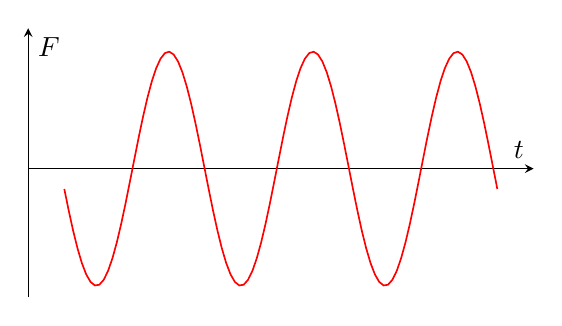
\begin{tikzpicture}
\begin{axis}[
    width=8cm, 
    height=5cm,
    axis x line=center, 
    axis y line=middle, 
    xlabel={$t$},
    ylabel={$F$},
    samples=100,
    ymin=-1.1, ymax=1.2,
    xmin=0, xmax=11,
    domain=0.25*pi:3.25*pi,
    ticks=none
]
\addplot [mark=none, semithick, red] {cos(2*deg(x)+10)};
\end{axis}
\end{tikzpicture}

}
\only<2>{\hfill 
\input{fig_tikz/multiharmonic_t_F}
}

\begin{itemize}[<+->]
 \item harmonische Anregung $F(t)=  F_C\cos\omega t + F_S\sin\omega t$ {\Large \color{green}\checkmark}
 \item allgemeine periodische Anregung $F(t+T)=F(t)$ \dots
\end{itemize}
\end{frame}

\begin{frame}
\frametitle{Vorgehensweise \normalsize{(nur für lineare Systeme)}}

\only<1>{
\begin{center}
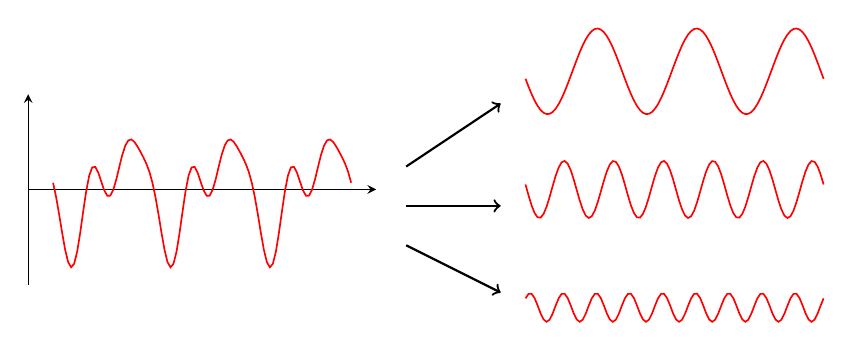
\begin{tikzpicture}
\begin{axis}[
    width=6cm, 
    height=4cm,
    axis x line=center, 
    axis y line=middle, 
    samples=100,
    ymin=-2, ymax=2,
    xmin=0, xmax=11,
    domain=0.25*pi:3.25*pi,
    ticks=none
]
\addplot [mark=none, semithick, red] {0.9*cos(2*deg(x)+10)-0.6*cos(4*deg(x)+80)+0.3*cos(6*deg(x)+40)};
\end{axis}
\begin{axis}[at={(6cm,1.5cm)},hide axis,
    width=6cm, 
    height=4cm,
    samples=100,
    ymin=-2, ymax=2,
    xmin=0, xmax=11,
    domain=0.25*pi:3.25*pi,
    ticks=none
]
\addplot [mark=none, semithick, red] {0.9*cos(2*deg(x)+10)};
\end{axis}
\begin{axis}[at={(6cm,0cm)},hide axis,
    width=6cm, 
    height=4cm,
    samples=100,
    ymin=-2, ymax=2,
    xmin=0, xmax=11,
    domain=0.25*pi:3.25*pi,
    ticks=none
]
\addplot [mark=none, semithick, red] {-0.6*cos(4*deg(x)+80)};
\end{axis}
\begin{axis}[at={(6cm,-1.5cm)},hide axis,
    width=6cm, 
    height=4cm,
    samples=100,
    ymin=-2, ymax=2,
    xmin=0, xmax=11,
    domain=0.25*pi:3.25*pi,
    ticks=none
]
\addplot [mark=none, semithick, red] {0.3*cos(6*deg(x)+40)};
\end{axis}
\draw[->, thick] (4.8, 1.5)--(6, 2.3);
\draw[->, thick] (4.8, 1.0)--(6, 1.0);
\draw[->, thick] (4.8, 0.5)--(6, -0.1);
\end{tikzpicture}


1. Schritt: Eingangssignal (Anregung) zerlegen
\end{center}
}

\only<2>{
\begin{center}
\input{fig_tikz/multiharmonic_synthesis}

2. Schritt: Teilprobleme lösen und deren Ausgangssignale (Antwort) addieren
\end{center}

}

\end{frame}

\input{v03sub_fourier_series}



\subsection{Allgemeine periodische Anregung}

\begin{frame}
\frametitle{Superpositionsprinzip}
\begin{center}
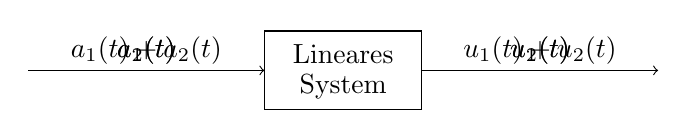
\begin{tikzpicture}
\draw (0, 0.21) node {Lineares};
\draw (0,-0.21) node {System};
\draw (-1,-0.5) rectangle (1, 0.5);
\draw[->] (-4, 0) -- (-1, 0);
\draw[->] ( 1, 0) -- ( 4, 0);
\draw[visible on=<1>] (-2.5, 0.25) node {$a_1(t)$};
\draw[visible on=<1>] ( 2.5, 0.25) node {$u_1(t)$};
\draw[visible on=<2>] (-2.5, 0.25) node {$a_2(t)$};
\draw[visible on=<2>] ( 2.5, 0.25) node {$u_2(t)$};
\draw[visible on=<3->] (-2.5, 0.25) node {$a_1(t)+a_2(t)$};
\draw[visible on=<3->] ( 2.5, 0.25) node {$u_1(t)+u_2(t)$};
\end{tikzpicture}

\end{center}
\uncover<3>{
Vorgehen für den (allgemein) periodisch erregten Einmassenschwinger 
\begin{align*}
a(t)&=\frac{1}{2}A_0 + \sum_{k=1}^{\infty} A_k \cos\left(\frac{2\pi kt}{T}\right) + B_k\left(\frac{2\pi kt}{T}\right)\\
&\approx\frac{1}{2}A_0 + \sum_{k=1}^{N} A_k \cos\left(\frac{2\pi kt}{T}\right) + B_k\left(\frac{2\pi kt}{T}\right)\\
u(t)&= \sum_{k=1}^{\infty} u_k(t) \approx \sum_{k=1}^{N} u_k(t)
\end{align*}
}
\end{frame}


\begin{frame}
\frametitle{Anwendungsbeispiel}
\begin{figure}
 \includegraphics[width=0.7\textwidth]{fig_img/earthquake_spectra.jpg}
 \caption*{Amplitudenspektrum ausgewählter Erdbeben \cite{amiri2008}}
\end{figure}
Anmerkung: Dieses Vorgehen wäre für Überschlagsrechnungen angebracht.

\end{frame}



\begin{frame}
\frametitle{Zusatzmaterial} % physical intution and complex representation
\vfill
\begin{center}
\includegraphics[width=0.2\textwidth]{fig_img/youtube.png}  

\href{https://www.youtube.com/watch?v=spUNpyF58BY}{\textsl{3Blue1Brown: Was ist eine Fourier-Transformation?}}
\end{center}  
\vfill
\end{frame}


%%%%%%%%%%%%%%%%%%%%%%%%%%%%%%%%%%%%%%%%%%%%%%%%

\section*{Literaturverzeichnis}

\begin{frame}[allowframebreaks]{}
	\printbibliography
\end{frame}


\end{document}
